\documentclass{article}
\usepackage[utf8]{inputenc}
\usepackage{setspace}
\usepackage[notes,backend=biber]{biblatex-chicago}
\bibliography{sources}
\usepackage[a4paper, total={6in, 8in}]{geometry}
\usepackage{mathtools}
\usepackage{graphicx}
\usepackage[section]{placeins}

\graphicspath{ {./images} }

\doublespacing
\linespread{2} %set line spacing

\nocite{*} % don't forget this shit, gave me a headache for an hour 

\begin{document}
\begin{titlepage}
\centering

{\LARGE\bfseries ECO475 Research Proposal}

\vspace{1cm}

Professor Ismael Mourifié

\vspace{1cm}

{\Large The Effect of Political Partisanship on Electric Vehicle Adoption in the US}

\vspace{2cm}

{\large Peter Shi}

January 30, 2023

\vfill

{\itshape University of Toronto}
\end{titlepage}

\newpage
\raggedright

\setlength{\parindent}{20pt}
\section{Introduction}

Transportation is one of the largest sources of greenhouse gas emissions, accounting for 27\% of greenhouse gas emissions in the US in 2020. Out of all transportation emissions, 57\% is attributable to light-duty vehicles. \autocite{EPA} Other pollutants from Internal Combustion Engines such as Particulate Matter, Nitrogen Oxides, and Carbon Monoxide are linked to adverse health outcomes such as asthma, reduced lung function, and cardiac and pulmonary mortality. \autocite{brugge_durant_rioux_2007} Thus the electrification of transportation, particularly personal electric vehicles (EVs) stands to both reduce carbon emissions and improve population health outcomes. However, despite sales doubling from 2020, EVs only made up 10\% of global new vehicle sales in 2021. \autocite{iea_2022} While EV sales have a strong upwards trend, it is still in the early stages of widespread adoption by the general public. Given the numerous positive externalities of EV adoption, many national governments have implemented incentive programs ranging from individual purchase subsidies to large spending packages for battery and charging infrastructure. \autocite{iea_2022} Additionally, factors affecting consumer adoption of EVs are a subject of ongoing study. This paper will focus on estimating the effect of political partisanship on EV adoption in the US using panel data while controlling for other factors explored in the literature.

\section{Literature Review}

An examination of two meta-analyses identifies a number of factors that influence EV adoption at a population level. Coffman et al. group adoption factors into two categories: internal and external. \autocite{coffman_bernstein_wee_2016} Anastasiadou and Gavanas alternatively group adoption factors according to the PESTLE framework—Political, Economic, Social, Technological, Legal, and Environmental factors. \autocite{anastasiadou_gavanas_2022} However, both studies cover the same set of factors. For the purposes of the summary, the grouping of Coffman et al. will be used. Internal factors are characteristics of the vehicle itself including acquisition and ownership costs, driving range, and charging time. External factors include fuel prices, consumer characteristics (including environmental beliefs), distances traveled, charging station networks, and public visibility. Policy mechanisms in the form of subsidies or infrastructure spending directly influence both internal and external factors of adoption.

However, the vast majority of the existing literature on factors affecting EV adoption and their effect sizes originates outside of economics, mostly coming from Transportation, Energy, and Sustainability studies. The economic literature on specific effects mostly focuses on the effects of fuel prices on adoption and finds a strong positive effect. \autocite{beresteanu_li_2011, gallagher_muehlegger_2011} More recent research supports these results, finding that gasoline prices have a larger effect on demand for electric vehicles (EVs) than electricity prices. \autocite{NBERw29842} Other economic research on specific factors affecting EV adoption comes almost exclusively from Muehlegger and Rapson who have studied the effects of EV subsidies to low and middle-income households. \autocite{NBERw25359} Their most comprehensive economic analysis on EV adoption does mention correlations between beliefs about climate change, adoption of sedans versus light trucks, and liberal versus conservative states, but the effect of climate change belief on EV adoption is not explicitly estimated since their paper focused on modeling future EV adoption scenarios.

Papers outside of economics have explored the relationship between political partisanship and EV subsidies, adoption, and general climate legislature in a limited capacity. Hayashida et al. found that governors and state legislatures were not significant for state EV subsidies but significant for household charger subsidies using a panel OLS model with controls and state and year fixed effects. \autocite{HAYASHIDA2021211} However, this study only explored the effect of state and not federal politics on EV subsidies and not the total effect on EV adoption as represented by vehicle population. Sintov et al. found that democrats were more likely to adopt EVs compared to their republican counterparts but the survey sample was quite small (N = 545) and unrepresentative of the population (Central Ohio) from which the survey was drawn. \autocite{SINTOV2020101576} Adua and Clark find a significant effect of political partisanship as measured by governorship and congressional delegation on state-level electric utility efficiency. \autocite{adua_clark_2020} But this effect may or may not translate to population-level EV adoption which occurs in a much more decentralized manner compared to electrical infrastructure. 

Given the review of the literature within and outside of economics, there is substantial room for estimating the effect size of partisanship in federal elections on EV adoption as measured by the proportion of the total vehicle population. 

\section{Data}

The primary dataset utilized for this paper is a monthly county-level panel of vehicle populations published by the State of Washington Department of Licensing. The dataset is grouped by vehicle class (passenger versus truck), drivetrain (battery-electric, hybrid-electric, and non-electric), and covers the time period from January 2017 to December 2022. 

Other variables include county-level demographic data (population, education, unemployment, and poverty) published by the Economic Research Service of the US Department of Agriculture, monthly fuel (gasoline) price data published by the US Energy Information Administration, 2017-2020 state-level Vehicle Miles Travelled Per Capita published by the Federal Highway Administration of the US Department of Transportation, and state-level purchase subsidies and county-level fueling/charging station numbers published by the Alternative Fuels Data Center of the US Department of Energy. Most importantly, county partisanship is measured by election returns in the 2016 and 2020 federal elections published by the MIT Election Data Lab. State-level governor and legislature partisanship controls are published by the National Governors Association and Ballotpedia respectively. 

Figure 1 shows the number of counties included in each observation month. The range is between 150-200 counties which represent roughly between 5\%-6\% of all US counties. Figure 2 shows the population counted in each observation month ranging from 93M - 103M people, representing between 27\%-30\% of the US population. Figure 3-6 shows the mean population, education, poverty, and unemployment in each observation month. Finally, Figure 7 shows the mean EV population in each county in each observation month.

\section{Model}

The proposed regression is the following OLS model:


${EV Proportion_{t,c}} = \alpha + \beta_{1} fed pol_{2016,c} + \beta_{2} \Delta fed pol_{2020,c} +\theta STATE POL_{t,s} +\delta  DEMOG_{c} + \kappa  INFRA_{t,c} + \nu  subsid_{t,s} + \omega fuelprice_{t} + \gamma_{t} + \tau_{s} +\epsilon$


Effect sizes of political partisanship are estimated with $\beta_{1}$ and $\beta_{2}$ which captures the effect of Republican vote share at a county level in the 2016 US federal election and the change in county vote share from 2016 to the 2020 election. $STATEPOL_{t,s}$ is a vector of state governor and legislature controls applied to the respective observation years. $DEMOG_{c}$ is a vector of county-level demographic controls from 2020 census data. $subsid_{t,s}$ controls for the effect of the count of EV subsidies at a state level at a particular time and $INFRA_{t,c}$ is a vector of controls for the number of fuel and charging stations at a county level at a particular time. Finally, $fuelprice_{t}$ controls for the monthly average price of gasoline for the observed time period. $\gamma_{t}$ and $\tau_{s}$ are a set of state and county fixed effects are added to further control for unobserved differences across time and states.

\newpage

\section{Figures}

\begin{figure}[!htb]
  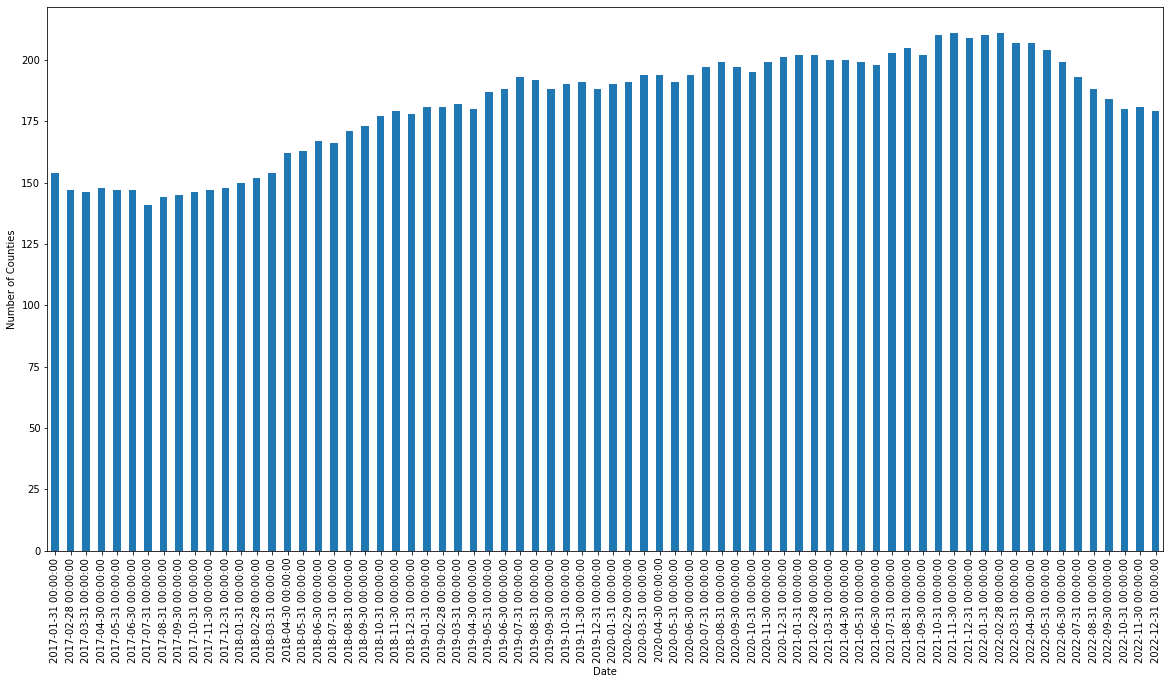
\includegraphics[width=\linewidth]{ncounties}
  \caption{Number of Counties counted over time}
\end{figure}

\begin{figure}[!htb]
  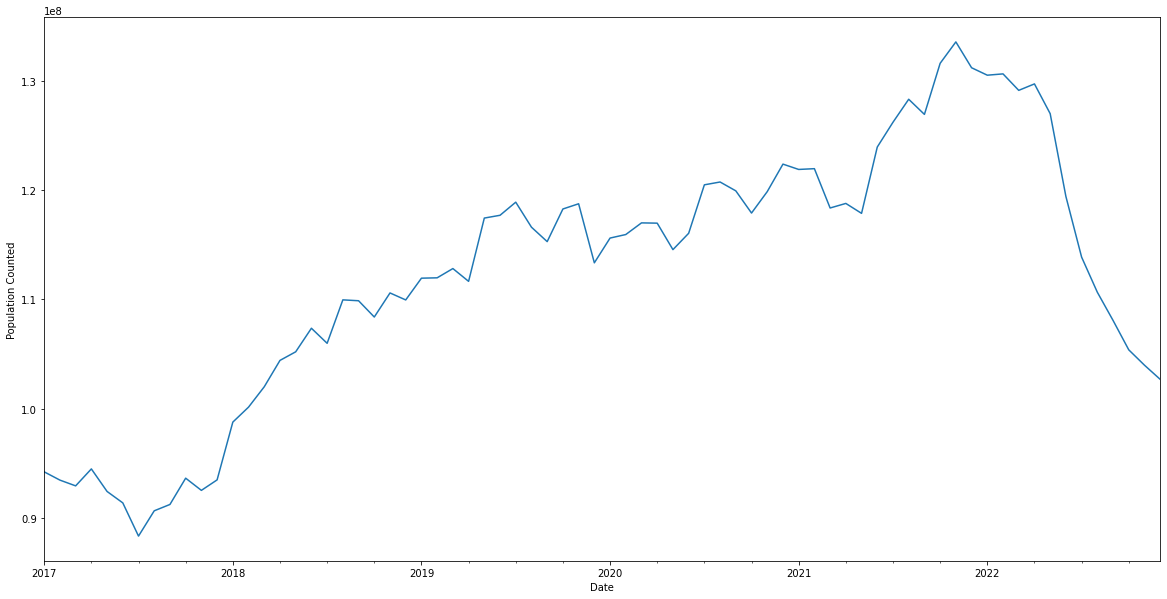
\includegraphics[width=\linewidth]{population}
  \caption{Population Counted}
\end{figure}

\begin{figure}[!htb]
  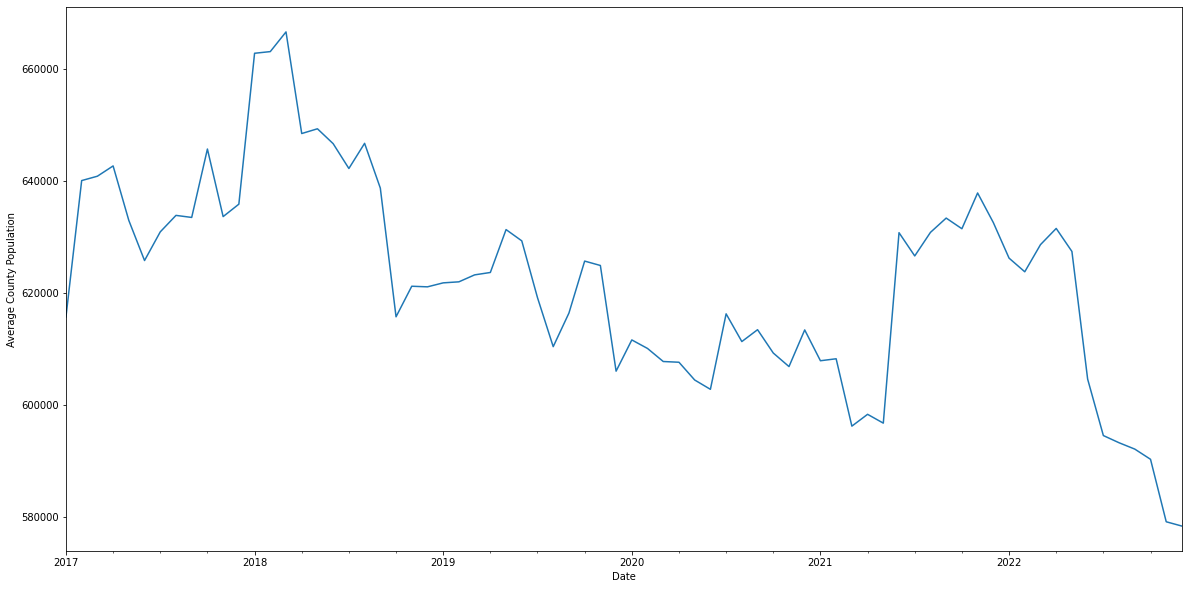
\includegraphics[width=\linewidth]{mean county population}
  \caption{Mean County Population}
\end{figure}

\begin{figure}[!htb]
  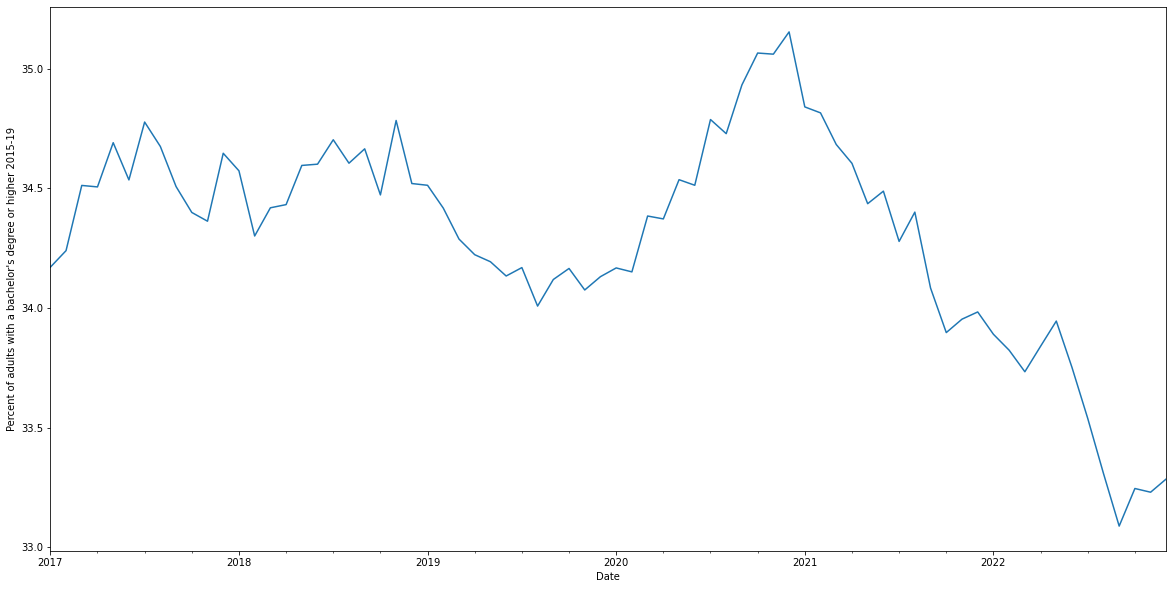
\includegraphics[width=\linewidth]{mean county educ}
  \caption{Mean County Education, Percent of Adults with a Bachelor's or Higher 2015-19}
\end{figure}

\begin{figure}[!htb]
  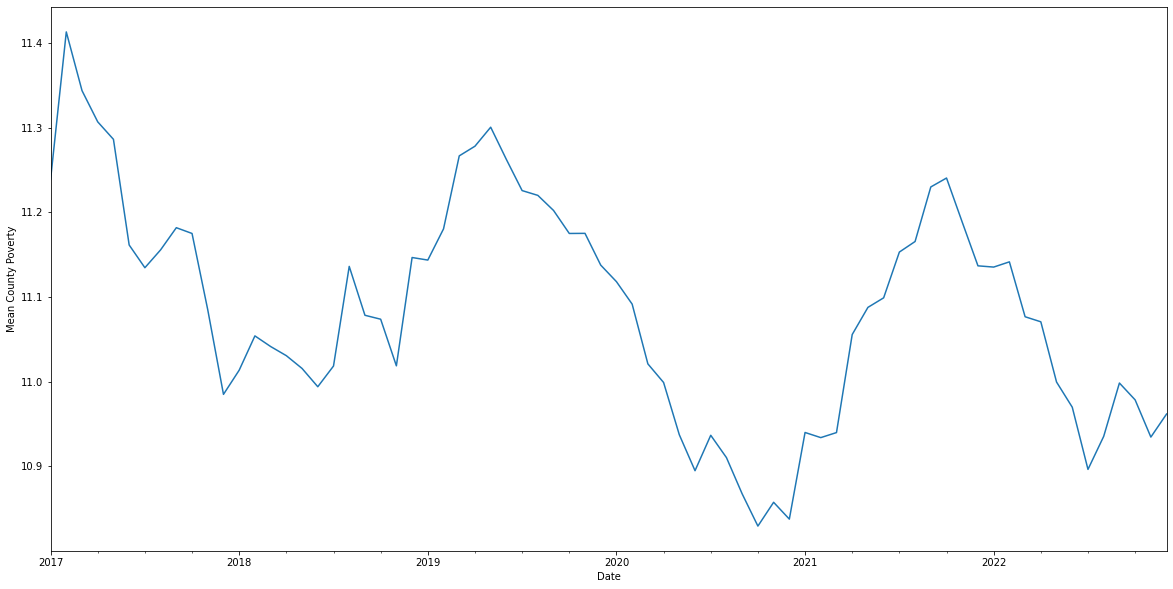
\includegraphics[width=\linewidth]{mean county pov}
  \caption{Mean County Poverty \%}
\end{figure}

\begin{figure}[!htb]
  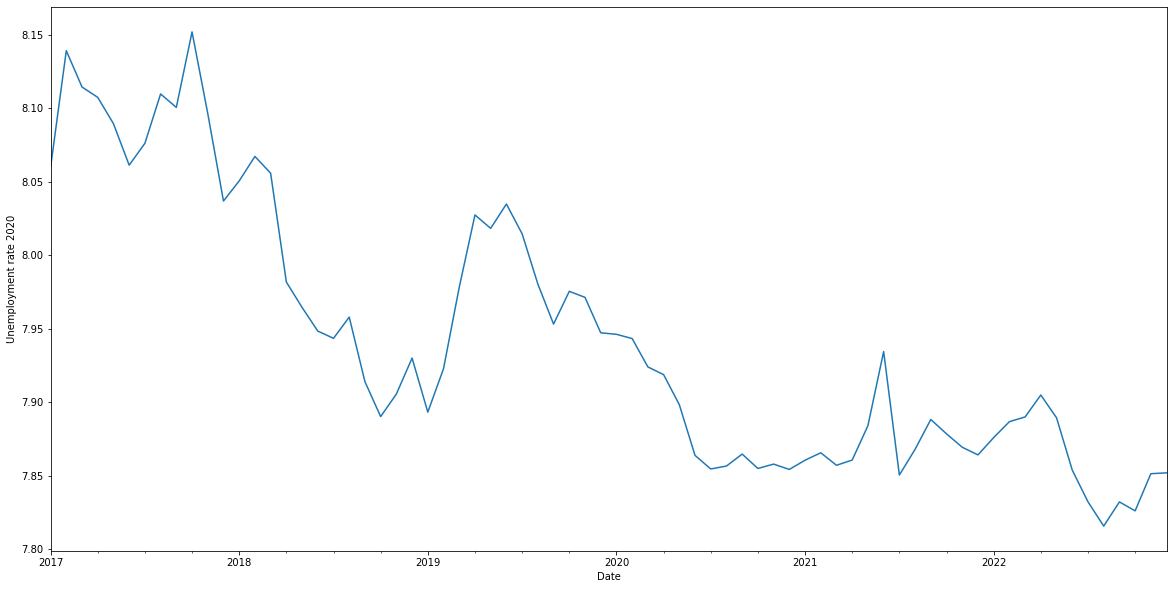
\includegraphics[width=\linewidth]{mean county unemp}
  \caption{Mean County Unemployment}
\end{figure}

\begin{figure}[!htb]
  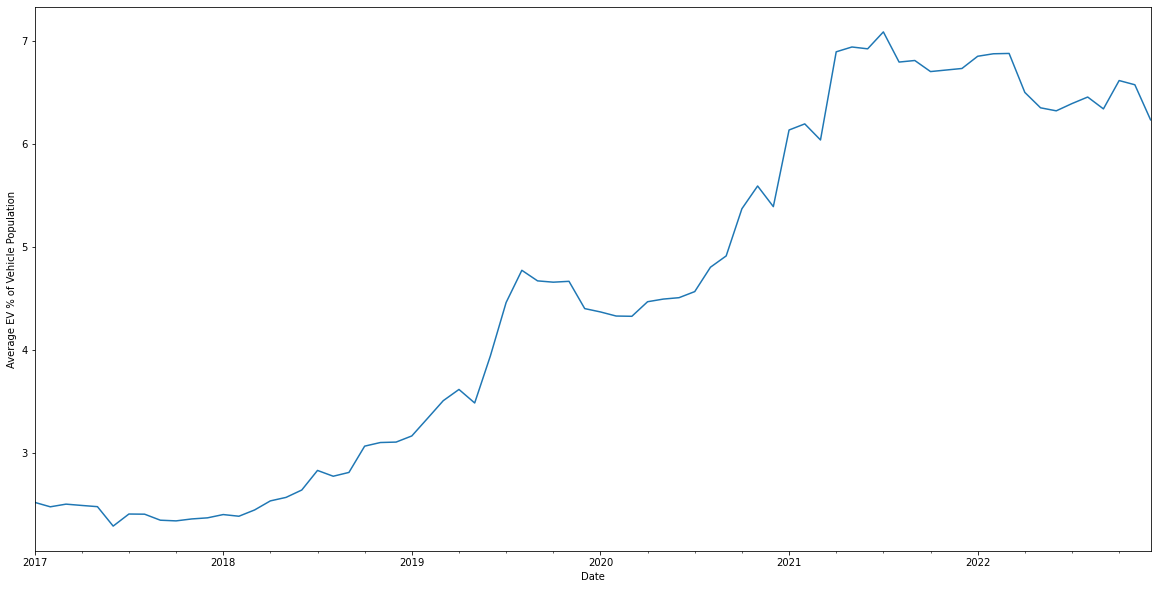
\includegraphics[width=\linewidth]{evpop}
  \caption{Average EV population as a \% of total vehicle population}
\end{figure}

\newpage

\printbibliography[
title={References}
]
\end{document}
